\chapter{METODOLOGI}
\section{Metode Pencarian Solusi Optimisasi}
  Untuk mencari solusi optimisasi pendeteksian objek kecil YOLOv7 yang terbaik, akan dilakukan penambahan atau perubahan \emph{bag-of-freebies}, \emph{bag-of-specials}, dan arsitektur YOLOv7.
  Setiap modifikasi-modifikasi itu akan diaplikasikan secara independen dan kombinatif.
  Yang dimaksud dengan kombinatif adalah modifikasi-modifikasi akan dikombinasikan menjadi 1 model YOLOv7.

  Setiap kombinasi modifikasi, independen atau tidak, akan diuji kemampuannya mendeteksi objek \emph{airborne}.
  Solusi optimisasi terbaik akan ditentukan berdasarkan metrik $AP_{50}$.
  Subbab \ref{section:modificationcandidates} akan membahas tentang kandidat modifikasi-modifikasi yang dapat dilakukan.

  Tahapan pencarian solusi optimisasi sendiri dapat dibagi menjadi enam tahap.
  Tahap-tahap tersebut adalah Persiapan Dataset, Pembuatan \emph{Auto-trainer}, Pembuatan Konfigurasi Modifikasi, \emph{Training Model}, Analisis, dan Pemilihan Model Terbaik.
  Urutan pengerjaan dari tahap-tahap ini dapat dilihat pada Gambar \ref{fig:metodologi}.
  \begin{figure}[H]
    \centering
    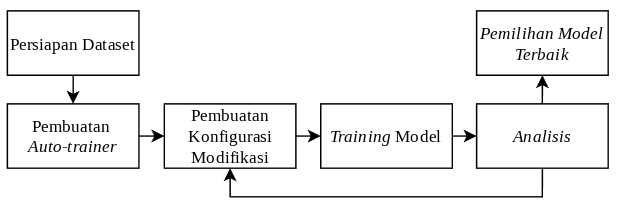
\includegraphics[scale=0.8]{figures/metodologi.png}
    \caption{Urutan Pengerjaan Penelitian}
    \label{fig:metodologi}
  \end{figure}
  \vspace{-1ex}
  %insert diagram modifikasi here
  %Menyiapkan dataset, Membuat \emph{auto-trainer}, Membuat konfigurasi-konfigurasi modifikasi, Melatih model-model YOLOv7 yang sudah dimodifikasi,
  %Menganalisis performa hasil modifikasi YOLOv7, dan Pemilihan model modifikasi YOLOv7 dengan skor mAP terbaik.

  Pada tahap persiapan dataset, akan dilakukan pengunduhan dataset dari \textcite{aot_dataset}.
  Gambar-gambar pada dataset ini kemudian akan di-\emph{sampling} dan didistribusikan menjadi dataset \emph{training}, validasi, dan pengujian.
  Pada pendistribusian dataset ini juga akan dilakukan \emph{balancing} antar kelas dan dataset positif negatif.
  \emph{Balancing} dilakukan agar tidak ada kelas yang mendominasi pada dataset.

  Selanjutnya, di tahap pembuatan \emph{auto-trainer}, akan dilakukan pembuatan program yang dapat dengan otomatis membangun dan melatih \emph{neural network} modifikasi YOLOv7.
  Pembuatan \emph{auto-trainer} ini dilakukan agar proses-proses pengerjaan tahapan-tahapan selanjutnya menjadi dapat dilakukan dengan lebih mudah.

  Setelah itu, akan dilakukan pembuatan konfigurasi-konfigurasi modifikasi.
  Konfigurasi modifikasi YOLOv7 akan dibuat agar dapat diinputkan pada \emph{auto-trainer}.
  Konfigurasi modifikasi akan berisi kombinasi modifikasi-modifikasi yang ada pada subbab \ref{section:modificationcandidates}.

  Tahapan selanjutnya adalah \emph{Training} model.
  Pada tahap ini, konfigurasi-konfigurasi modifikasi pada tahapan sebelumnya akan dibangun dan kemudian dilatih.
  Model akan dilatih \emph{from scratch}. Dengan kata lain, model tidak akan dilatih dengan menggunakan \emph{pre-trained weights}.
  Hasil dari tahap ini adalah \emph{weights neural network} modifikasi YOLOv7, histori pelatihannya, dan metrik-metriknya pada dataset uji.

  Pada tahap analisis, hasil dari tahap sebelumnya akan dianalisis untuk mencari tahu performa model-model hasil modifikasi.
  Analisis juga dilakukan untuk menemukan \emph{gap} kandidat modifikasi lain yang masih bisa dieksplorasi untuk meningkatkan kemampuan pendeteksian objek kecil YOLOv7.
  Ketika suatu kandidat modifikasi seperti itu ditemukan, maka akan dilakukan kembali pembuatan konfigurasi modifikasi untuk menguji kandidat modifikasi baru tersebut.

  Tahapan terakhir adalah pemilihan model terbaik.
  Pada tahapan ini akan dipilih model yang memiliki performa terbaik dari antara model-model hasil modifikasi lainnya.
  Pemilihan model akan dilakukan dengan berdasarkan pada skor mAP tertinggi.
  Untuk mempertahankan solusi optimisasi yang dapat melakukan deteksi secara \emph{real time}, model yang akan dipilih adalah model yang dapat melakukan deteksi yang cukup cepat pada \emph{edge} GPU.


\section{Kandidat Modifikasi}
\label{section:modificationcandidates}
  \subsection{Augmentasi Mosaik}
    Seperti yang dibahas pada subbab \ref{section:mosaic_study}, augmentasi mosaic pada dataset mampu meningkatkan akurasi deteksi objek-objek kecil dari model.
    Oleh karena itu, akan dilakukan eksperimen menambahkan augmentasi mosaik pada YOLOv7 untuk melihat apakah augmentasi ini akan meningkatkan akurasi, khususnya pada dataset objek kecil.
  \subsection{Rekalkulasi \emph{Anchor}}
    %Yang dimaksud dengan rekalkulasi \emph{anchor on-training}  adalah ketika ukuran-ukuran \emph{anchor box} direkalkulasi pada saat training.
    %Berbeda dengan \emph{clustering pre-training} seperti pada YOLOv2 \parencite{yolov2}, ukuran-ukuran \emph{anchor} akan di-\emph{learning} bersama dengan pendeteksi objeknya.
    %Untuk melakukan hal ini, digunakan algoritma optimisasi \emph{anchor box} yang mirip dengan algoritma \textcite{anchoropt}.
    %Pada bagian \emph{head}, akan ditempelkan suatu layer yang akan mengoutputkan faktor \emph{rescaling} dari tiap \emph{anchor box}.
    %Bagian tersebut akan di-\emph{training} bersama dengan YOLOv7 \emph{anchor box} akan teroptimisasi tidak hanya pada dataset, namun pada keseluruhan \emph{neural network} juga.
    Anchor yang disediakan pada kode implementasi dari YOLOv7 merupakan anchor yang dikalkulasi untuk mengoptimisasi deteksi pada dataset
    COCO2017. Dengan pertimbangan bahwa distribusi dataset yang akan digunakan pada penelitian ini berbeda dari objek general di COCO2017,
    maka anchor harus direkalkulasi. Dengan melakukan rekalkulasi anchor, tiap layer head pada YOLOv7 akan dengan lebih mudah mem-\emph{fit}
    objek-objek yang ada pada gambar.

    \subsection{Menggunakan \emph{Localization Loss Extended IoU} }
      \emph{Extended} IoU (EIoU) merupakan salahsatu modifikasi dari
      IoU yang dibuat untuk menyelesaikan permasalahan \emph{vanishing gradient}
      pada IoU \parencite{eiou}. Hal yang menyebabkan IoU bermasalah dengan \emph{vanishing gradient}
      adalah nilai dari IoU yang selalu menjadi 0 ketika 2 \emph{bounding box} tidak beririsan.
      Permasalahan ini diselesaikan oleh EIoU dengan memberikan nilai negatif untuk 
      bounding box yang tidak beririsan, sehingga neural network dapat mengoptimasi loss function $-EIoU$.
      Teknik konveksikasi juga dapat dilakukan dengan mengoptimasi $(1-EIoU)^2$

      YOLOv7 sendiri menggunakan CIoU sebagai localization loss. CIoU juga merupakan suatu solusi
      dari permasalahan \emph{vanishing gradient}. CIoU menambahkan suku jarak antar bounding box 
      dan kecocokan \emph{aspect ratio} antar boundingbox pada IoU. Keunggulan EIoU daripada CIoU
      adalah EIoU akan bertingkah seperti IoU ketika bounding box beririsan. Karena metrik-metrik
      yang digunakan untuk mengukur kemampuan deteksi dilakukan berdasarkan IoU, dianggap akan
      lebih baik jika loss yang digunakan sama seperti metriknya \parencite{eiou}.

  \subsection{Modifikasi Koneksi Neck pada Backbone}
    %\begin{figure}[ht]
    %  \centering
    %  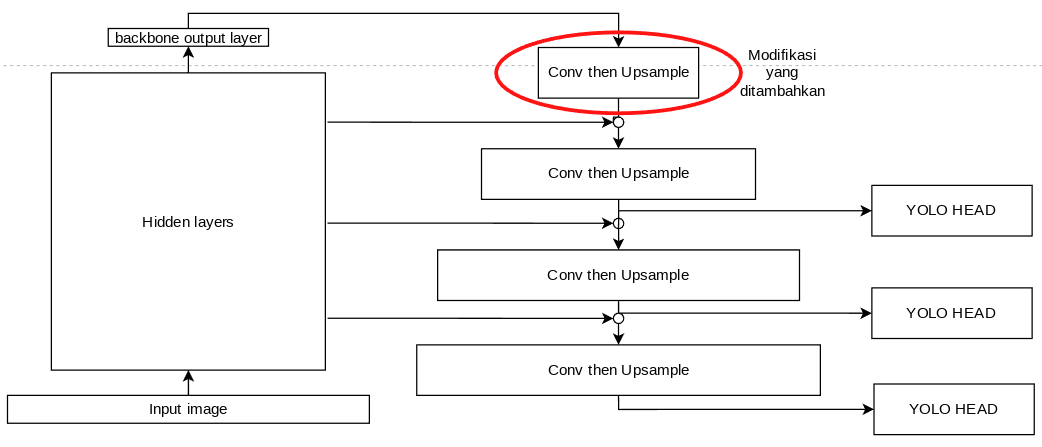
\includegraphics[scale=0.5]{figures/add-more-upsampling.png}
    %  \caption{Menambah \emph{upsampling} pada \emph{neck}}
    %  \label{fig:neckaddupsampling}
    %\end{figure}
    \begin{figure}[H]
      \centering
      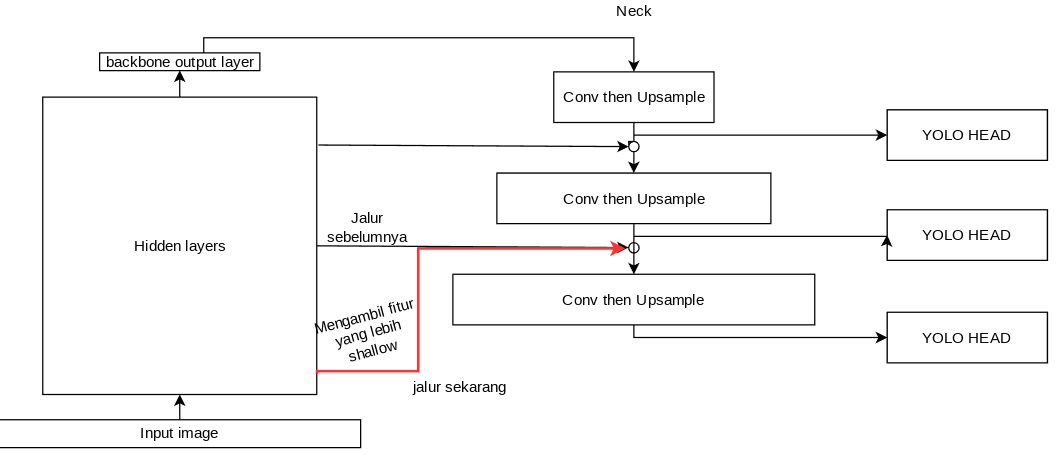
\includegraphics[scale=0.5]{figures/neck-move-back.png}
      \caption{Menggunakan \emph{feature map} dari layer yang lebih di belakang}
      \label{fig:neckmoveback}
    \end{figure}
    Seperti pada penelitian-penelitian terkait di subbab \ref{section:relatedwork}, modifikasi \emph{neck} dapat dilakukan untuk meningkatkan akurasi pendeteksian objek kecil.
    Modifikasi koneksi \emph{neck} ke \emph{backbone} dapat dilakukan dengan memindahkan sumber feature map untuk beberapa layer neck lebih jauh ke belakang seperti pada Gambar \ref{fig:neckmoveback}.
    %Penambahan layer upsampling dapat membuat neural network untuk mendapatkan feature-map yang lebih detail sehingga dapat melakukan pendeteksian objek kecil dengan lebih baik.
    Pemindahan sumber feature map ke belakang dapat dilakukan untuk mengantisipasi fitur objek kecil yang bisa saja hilang ketika layer neural network semakin dalam.
    Dengan memindahkannya lebih ke belakang, YOLOv7 akan melakukan deteksi dengan memanfaatkan fitur yang abstraksi yang lebih rendah tetapi sedikit informasi yang hilang.
  \subsection{Penambahan YOLO Head}
    \begin{figure}[H]
      \centering
      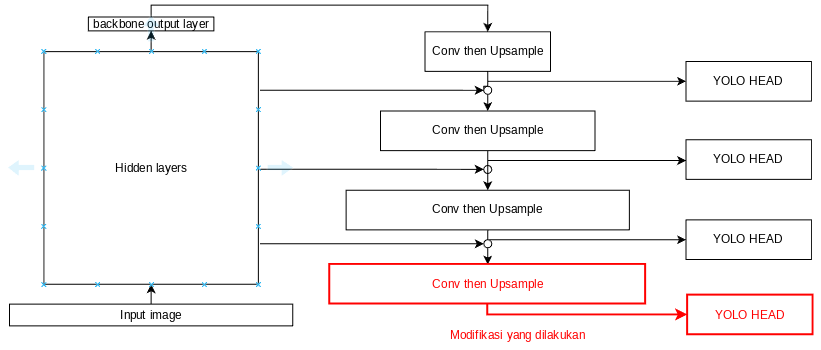
\includegraphics[scale=0.65]{figures/addmorehead.png}
      \caption{Penambahan \emph{Layer} Head pada YOLO}
      \label{fig:addmorehead}
    \end{figure}
    Penambahan YOLO head dapat membuat YOLOv7 melakukan deteksi pada skala yang lebih banyak.
    Hal ini akan berpengaruh pada kemampuan pendeteksian objek kecil.
    Dengan melakukan pendeteksian pada skala yang lebih banyak, YOLOv7 dapat mendeteksi objek yang besar maupun kecil.
    %Perhatikan bahwa penambahan YOLO Head akan diikuti dengan penambahan \emph{layer upsampling} pada \emph{neck} seperti di Gambar \ref{fig:addmorehead}.

  \subsection{Mengganti YOLO Head menjadi \emph{Decoupled Anchor-free Head}}
    \begin{figure}[H]
      \centering
      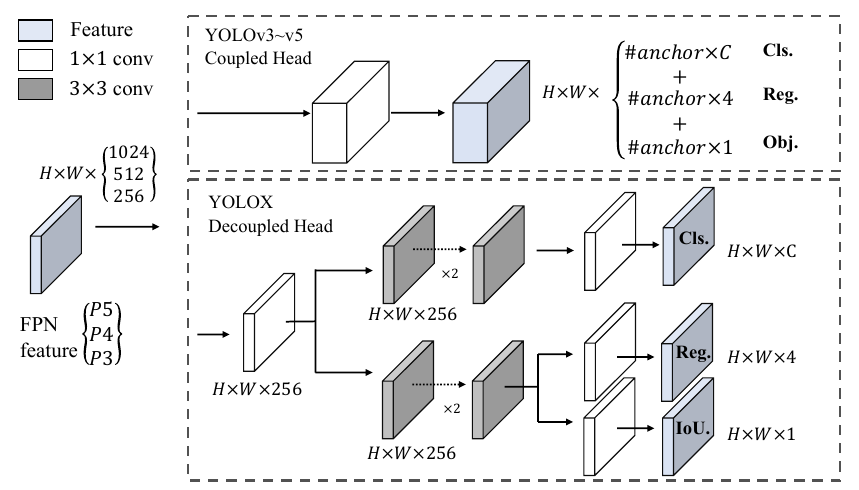
\includegraphics[width=0.8\textwidth]{figures/anchorfree-yolox.png}
      \caption{\emph{Decoupled Anchor-free Head} pada YOLOX \parencite{yolox}}
      \label{fig:anchorfree}
    \end{figure}

    Pada YOLOX, \emph{coupled anchor head} seperti pada arsitektur YOLO pada umumnya diganti dengan \emph{decoupled anchor-free head} \parencite{yolox}.
    Keuntungan dari model anchor-free adalah kita tidak perlu mendefinisikan \emph{anchor} sebelum melakukan training sehingga mengurangi beberapa proses
    tuning heuristik seperti rekalkulasi anchor. Memakai \emph{head} yang anchor free juga memberi kompleksitas proses training dan pendekodean output model.
    \cite{yolox} melaporkan peningkatan pada akurasi dan pengurangan parameter sehingga mempercepat lama deteksi.
    Oleh karena hal-hal tersebut, mencoba memakai \emph{head anchor-free} di YOLOv7 baik untuk dicoba.
    
    
\section{Dataset}
\label{section:dataset}

  \subsection{Sumber Dataset}
    Dataset untuk objek-objek \emph{airborne} didapatkan dari \textcite{aot_dataset} dan dihost pada suatu server AWS S3 Bucket.
    Dataset ini berisi video-video monokromatik penerbangan UAV.
    Terdapat 4 kelas pada dataset ini yaitu pesawat, helikopter, burung, dan \emph{other}.
    Distribusi dataset training dan uji dapat dilihat pada tabel \ref{tbl:datasettraintest} sedangkan distribusi kelas dari dataset dapat dilihat pada Tabel \ref{tbl:datasetclasses}.
    
\begin{table}[H]
  \centering
  \captionof{table}{Distribusi Dataset Training dan Test}
  \label{tbl:datasettraintest}
  \begin{tabular}{|c|c|c|c|c|}
    \hline
    Pembagian & Ukuran (TB) & Sekuen penerbangan & Jumlah Gambar & Jumlah Label\\
    Dataset &  & UAV &  & \\
    \hline
    Training & 11,3 & 4154 & 4975765 & 2891891\\
    \hline
    Validation + Test &2.1 &789 & 943852 & 496075\\
    \hline
    Total &13,4 &4943 & 5919617 & 3387966\\
    \hline
  \end{tabular}
\end{table}
    \begin{tabular}{ c c c c c c }
  \toprule[1.5pt]
  Splits & Total Objects & Airplane & Helicopter & Bird & \emph{Other 4 Classes}\\
  \midrule
  Training & 2,89 M & 0,79 M& 1,22 M& 0,33 M& 0,54 M\\
  Validation + Test &0,50 M &0,13 M & 0,17 M&0,06 M&0,14 M\\
  \midrule
  Total &3,39 M &0,92 M & 1,39 M&0,39 M&0,69 M\\
  \bottomrule[1.5pt]
\end{tabular}
  
  \subsection{Sampling Dataset}
    Karena jumlah dataset pada \textcite{aot_dataset} berukuran sangat besar, dan keterbatasan
    \emph{computational resource}, hanya sebagian dari dataset tersebut akan digunakan untuk \emph{training} dan \emph{test}.
    Akan diambil total 700 gambar dari dataset dengan pembagian sesuai dengan Tabel \ref{tbl:datasetsamplingdist}
    \begin{table}[h]
      \centering
      \captionof{table}{Distribusi Sampling Dataset}
      \label{tbl:datasetsamplingdist}
      \begin{tabular}{|c|c|c|c|c|c|c|}
        \hline
        Pembagian &Total & \multicolumn{4}{c}{Presentase}&\\
                           \cline{2-7}
                  &Gambar& Pesawat & Helikopter & Burung & Drone & Negatif\\
        \hline
        Training  &400 &23,75\%  &23,75\%     &23,75\% &23,75\%       &5\%\\
        \hline                                              
        Validation&100  &20\%     &20\%        &20\%    &20\%          &20\%\\
        \hline                                                           
        Test      &200  &20\%     &20\%        &20\%    &20\%          &20\%\\
        \hline
      \end{tabular}
    \end{table}

    %Untuk membagi dataset agar terdistribusi seperti pada Tabel \ref{tbl:datasetsamplingdist}, akan digunakan algoritma seperti berikut:
    %\begin{algorithmic}
    %  \State $L_0 \gets$ List index gambar-gambar yang memiliki objek kelas pesawat
    %  \State $L_1 \gets$ List index gambar-gambar yang memiliki objek kelas helikopter
    %  \State $L_2 \gets$ List index gambar-gambar yang memiliki objek kelas burung 
    %  \State $L_3 \gets$ List index gambar-gambar yang memiliki objek kelas \emph{Other}
    %  \State $L_4 \gets$ List index gambar-gambar yang memiliki objek kelas negatif
    %  \For{$i \gets 0$ to $4$}
    %    \State $L_i \gets shuffle(L_i)$
    %  
    %  

    %\end{algorithmic}

\section{Instrumen dan \emph{Setup} Eksperimen}
  Untuk melaksanakan eksperimen ini, akan digunakan suatu komputer yang dilengkapi dengan
  GPU Nvidia RTX 2080 Ti yang memiliki kapasitas 11GB VRAM. Oleh karena keterbatasan ini,
  Melatih model-model YOLOv7 besar seperti W6, E6, dan E2E yang dimodifikasi menjadi sangat sulit,
  apalagi pada skala input sesuai dengan dimensi dataset.
  Oleh karena hal ini, arsitektur yang akan dipilih sebagai \emph{baseline} modifikasi adalah YOLOv7 dengan
  ukuran normal karena model tersebut adalah model terbesar yang mampu di-\emph{train} pada RTX 2080 Ti dengan 
  input size 1600x1600 dan batch size 1.

  Selain itu, jumlah dataset yang akan digunakan juga akan dibatasi menjadi 400 seperti pada subbab \ref{section:dataset} untuk menghemat waktu training.
  Pada pilot test, ditemukan bahwa dibutuhkan sekitar 20 jam untuk men-\emph{train} model sebanyak 300 epoch pada dataset dengan 400 gambar jika menggunakan
  GPU RTX 2080 Ti.





%\section{Skema Training Model}
%  Untuk melatih berbagai modifikasi YOLOv7, akan dibuat suatu \emph{auto-trainer}.
%  \emph{Auto-trainer} ini akan menerima suatu \emph{file} konfigurasi modifikasi YOLOv7, dan dengan otomatis membangun arsitektur YOLOv7 yang termodifikasi dan melatihnya.
%  Setelah mendapatkan model modifikasi YOLOv7 yang sudah dilatih, \emph{auto-trainer} akan menguji model tersebut dengan dataset uji.
%  Metrik-metrik pengujian, grafik histori \emph{training loss vs validation loss}, dan \emph{weights} dari model kemudian akan dikirim ke user.
%  Dengan membuat \emph{auto-trainer} ini, proses pelatihan model dan pelaporan hasil menjadi terotomasi sehingga akan mempermudah proses penelitian.
%
%\section{Timeline Pelaksanaan Penelitian}
%  \newcommand{\w}{}
%  \newcommand{\G}{\cellcolor{gray}}
%  \begin{table}[h!]
%    \captionof{table}{Tabel timeline}
%    \label{tbl:timeline}
%    \begin{tabular}{|p{3.5cm}|c|c|c|c|c|c|c|c|c|c|c|c|c|c|c|c|}
%  
%      \hline
%      \multirow{2}{*}{Kegiatan} & \multicolumn{16}{|c|}{Minggu} \\
%      \cline{2-17} &
%      1 & 2 & 3 & 4 & 5 & 6 & 7 & 8 & 9 & 10 & 11 & 12 & 13 & 14 & 15 & 16 \\
%      \hline
%  
%      % Gunakan \G untuk mengisi sel dan \w untuk mengosongkan sel
%      Persiapan Dataset &
%      \G & \w & \w & \w & \w & \w & \w & \w & \w & \w & \w & \w & \w & \w & \w & \w \\
%      \hline
%  
%      Pemb. \emph{Auto-trainer} &
%      \w & \G & \w & \w & \w & \w & \w & \w & \w & \w & \w & \w & \w & \w & \w & \w \\
%      \hline
%  
%      Pemb. Konfigurasi&
%      \w & \w & \G & \G & \G & \G & \G & \G & \G & \G & \G & \G & \w & \w & \w & \w \\
%      Modifikasi &
%      \w & \w & \G & \G & \G & \G & \G & \G & \G & \G & \G & \G & \w & \w & \w & \w \\
%      \hline
%  
%      Training Model &
%      \w & \w & \G & \G & \G & \G & \G & \G & \G & \G & \G & \G & \w & \w & \w & \w \\
%      \hline
%
%      Analisis &
%      \w & \w & \G & \G & \G & \G & \G & \G & \G & \G & \G & \G & \G & \w & \w & \w \\
%      \hline
%
%      Pemb. Laporan &
%      \w & \w & \w & \w & \w & \w & \w & \w & \w & \w & \w & \w & \G & \G & \G & \G \\
%      \hline
%  
%    \end{tabular}
%  \end{table}
